\setcounter{chapter}{1}
\chapter{ÉTUDE PRÉLIMINAIRE}
\minitoc %insert la minitoc
\graphicspath{{Chapitre2/figures/}}

%\DoPToC

%==============================================================================
\pagestyle{fancy}
\fancyhf{}
\fancyhead[R]{\bfseries\rightmark}
\fancyfoot[R]{\thepage}
\renewcommand{\headrulewidth}{0.5pt}
\renewcommand{\footrulewidth}{0pt}
\renewcommand{\chaptermark}[1]{\markboth{\MakeUppercase{\chaptername~\thechapter. #1 }}{}}
\renewcommand{\sectionmark}[1]{\markright{\thechapter.\thesection~ #1}}

\begin{spacing}{1.5}

%==============================================================================
\section*{Introduction}
Après avoir présenté le cadre général de notre projet et le cœur du sujet, nous entamons par le biais de ce chapitre une étude théorique, préface à sa réalisation. L'étude de l'existant sera l'opportunité de présenter plus en détail la problématique rencontrée. Une mise au point sur l'état des lieux de la gestion de projets du côté des clients de l'entreprise attestera de l'intérêt du projet pour un usage externe à l'entreprise. Enfin, une vue d'ensemble de solutions similaires présentes sur le marché permettra de se faire une idée globale sur les fonctionnalités à attendre du produit.

%==============================================================================
\section{Étude de l'existant}
L'étude de l'existant permet d'identifier les points forts ainsi que les points faibles de la démarche existante. Cette étude permettra de bien cibler les besoins de l'entreprise, en vue d'en tenir compte lors de la conception et du développement de la solution.
%-----------------------------------------------------------------------------------
\subsection{Description de l'existant}
La démarche de gestion de projet actuelle se base sur l'utilisation du logiciel Excel pour générer des documents associés aux différentes activités d'un projet. En effet, le chef de projet répertorie chaque catégorie d'artéfact associée à la gestion d'un projet sous forme de tableur Excel. Il procède ainsi à l'ajout et l'édition d'entrées pour chaque catégorie d'artéfact et y indique l'ensemble des informations requises. Cette procédure est facilitée par la duplication de fiches Excel de base, vierges, préparées à l'avance pour chaque catégorie. Ainsi, pour chaque catégorie d'artéfact; l'ensemble des entêtes et des valeurs prédéfinies pour chaque champs y est déja déclaré. La table d'entrées est accompagnée d'un ensemble d'indicateurs, statiques et dynamiques, pertinents à la catégorie en question. On y retrouve également les logos de l'entreprise IT SERV et du client porteur de projet. Des exemples de ces fiches sont exposés aux figures \ref{fig:risqueFiche} et \ref{fig:actionFiche}, traitant respectivement des artéfacts risques et actions pour un projet.

\begin{figure}[H]
\centering
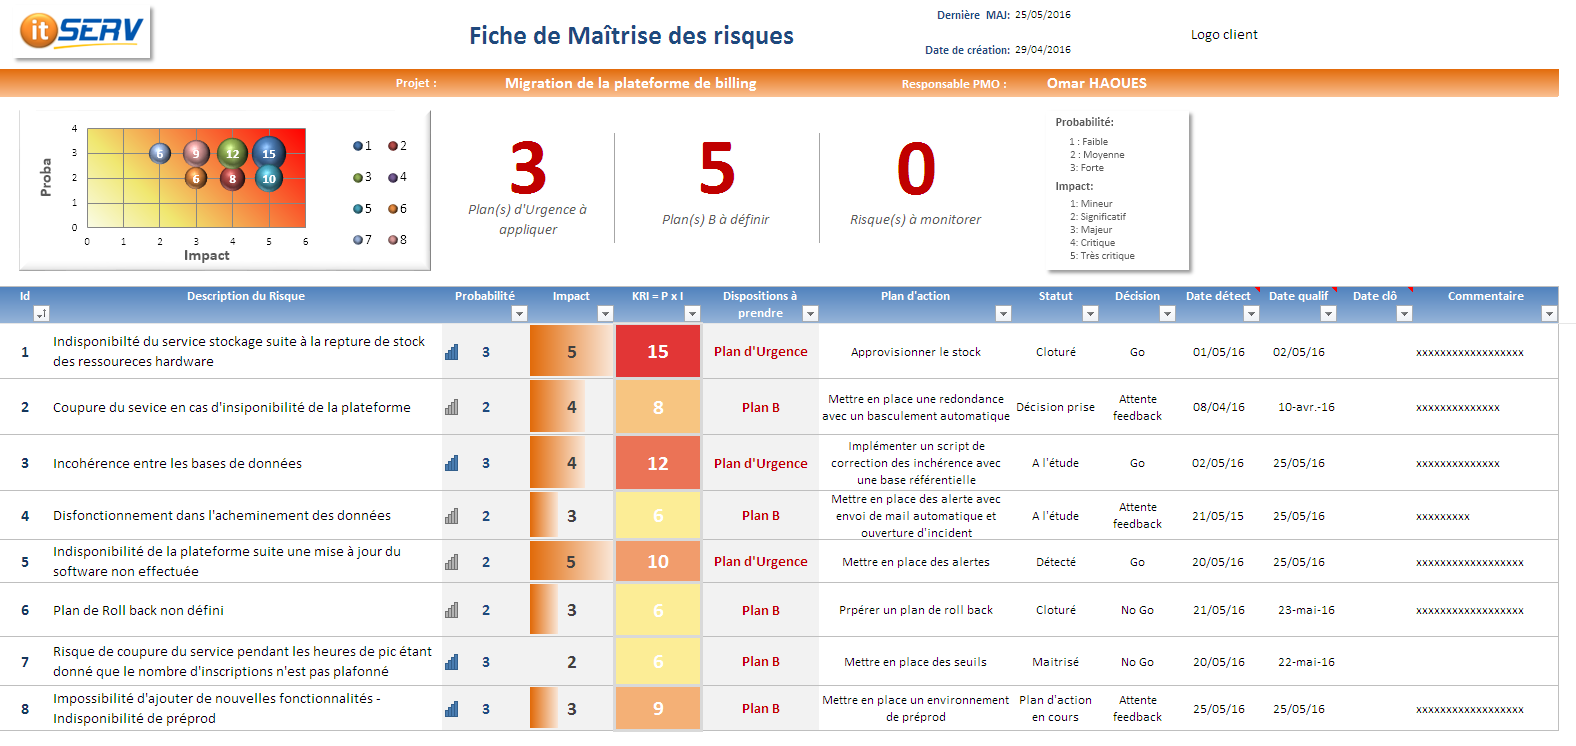
\includegraphics[width=\textwidth]{ficheRisques.png}
\caption{Exemple d'une fiche de maîtrise des risques}
\label{fig:risqueFiche}
\end{figure}

\begin{figure}[H]
\centering
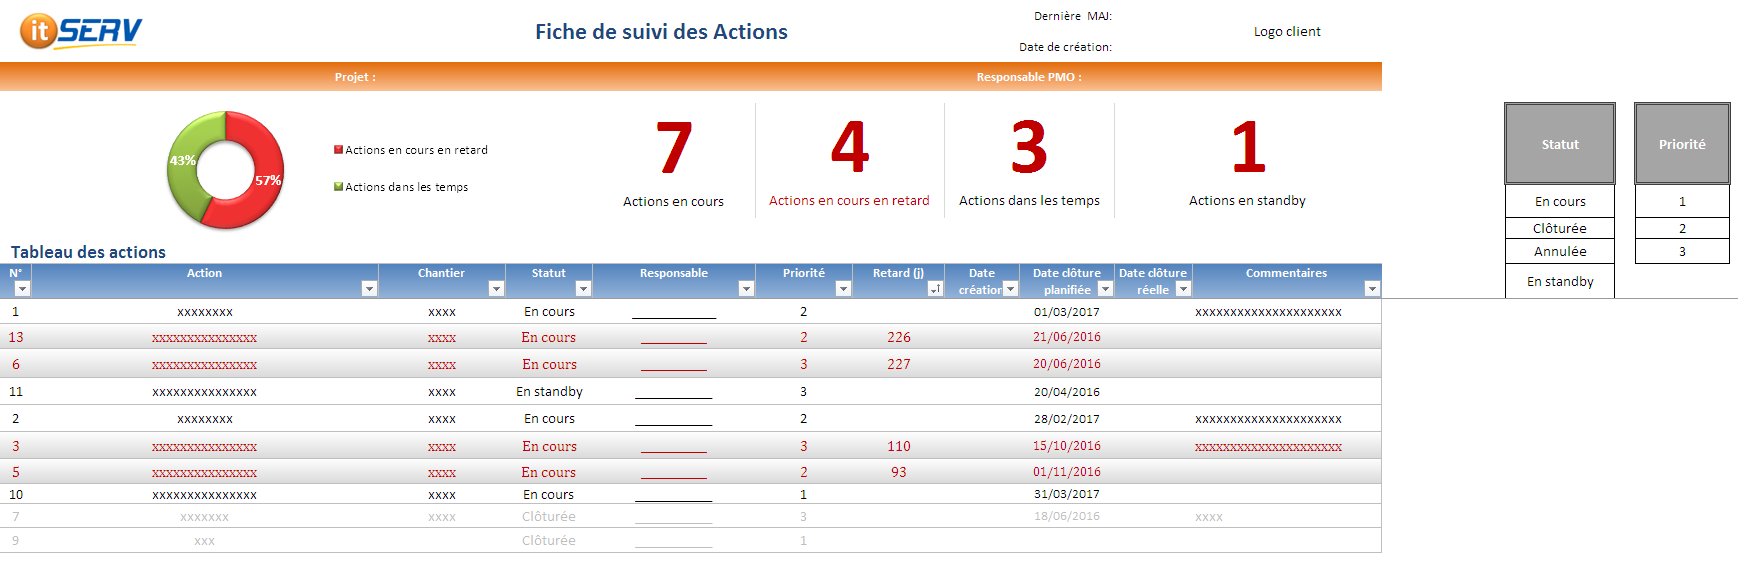
\includegraphics[width=\textwidth]{ficheActions.png}
\caption{Exemple d'une fiche de suivi des actions}
\label{fig:actionFiche}
\end{figure}
\

Le chef de projet est régulièrement chargé de diffuser les mises à jour relatives à un projet, périodiquement ou à la demande, au travers de l'envoi de messages électroniques directement aux parties concernées.\\

Cette méthode de travail possède certains atouts, mais dissimule dans l'ensemble plusieurs inconvenances qui nuisent à son niveau d'efficacité et à la performance de la gestion de projets par l'entreprise. Ces points sont exposés dans la section suivante.

%-----------------------------------------------------------------------------------
\subsection{Critique de l'existant}
La présentation de la méthode de gestion actuelle nous permet de déceler des limitations importantes, inhérentes à la démarche générale.\\
\\
Reconnaissons tout d'abord les mérites non négilgeables de celle-ci, à savoir :
\begin{itemize}
    \item Disponibilité de fiches de base, contraignant les champs à choix retraints aux options prédéfinies
    \item Présence de champs autocalculés ainsi que de supports visuels, assistant le client dans la compréhension de certains champs, dont la signification peut s'avérer obscure
    \item Génération automatique d'indicateurs riches (statistiques numériques, graphiques en camembert, ...)
\end{itemize}
\

Outre ces quelques bénéfices, cette méthode de gestion présente les nombreuses limitations suivantes :
\begin{itemize}
    \item \textbf{Perte en productivité} : induite d'un déficit d'automatisation de la démarche de gestion des fichiers
    \item \textbf{Fragmentation des données} : les données relatives à chaque projet sont réparties, sous forme d'une multitude de documents, souvent désorganisés
    \item \textbf{Journalisation non fiable des mises à jour} : la responsaibilité de celle-ci relève entièrement de l'oraganisation choisie par le chef de projet, et requiert un effort manuel, exclusivement dédié à la tâche
    \item \textbf{Traçabilité impossible} : l'origine des modifications des fichiers n'est pas connue
    \item \textbf{Stockage inneficace} : problème de centralisation pour de l'ensemble des données des projets menés par l'entreprise, redondance de données, oraganisation manuelle, ...
    \item \textbf{Sécurité non garantie} : la sécurisation des données est entièrement à la charge des parties prenantes y ayant accès
    \item \textbf{Condifentailité diffciele à assurer} : elle implique en pratique l'édition soigneuse, au cas par cas, des fichiers partagés
    \item \textbf{Synthèse des données impossible} : impossible de se reposer fiablement sur les données des fichiers pour les besoins d'aide à la décision de l'entreprise (dû aux problèmes susmentionnés)
    \item \textbf{Collaboration fastidieuse} : contribution d'intervenants non gérée par la solution actuelle. Le chef de projet transforme individuellement tous les flux d'information en données, avant de les indiquer dans le fichier approprié
\end{itemize}
\

Ce nombre abondant de limitations impose pour l'entreprise une révolution dans sa méthode actuelle de gestion de projets. Notre projet a pour but de fournir une solution adéquate à l'ensemble de ces lacunes. La solution à concevoir aspire ainsi à combiner les points forts de la démarche existante tout en apportant une solution efficace à ses problèmes inhérents.


%==============================================================================
\section{Étude des solutions disponibles sur le marché}
%-----------------------------------------------------------------------------------
\subsection{Présentation des solutions existantes}

%-----------------------------------------------------------------------------------
\subsection{Critique des solutions existantes}



%==============================================================================
\section*{Conclusion}


%==============================================================================
\end{spacing}
